% Options for packages loaded elsewhere
\PassOptionsToPackage{unicode}{hyperref}
\PassOptionsToPackage{hyphens}{url}
%
\documentclass[
]{article}
\usepackage{amsmath,amssymb}
\usepackage{iftex}
\ifPDFTeX
  \usepackage[T1]{fontenc}
  \usepackage[utf8]{inputenc}
  \usepackage{textcomp} % provide euro and other symbols
\else % if luatex or xetex
  \usepackage{unicode-math} % this also loads fontspec
  \defaultfontfeatures{Scale=MatchLowercase}
  \defaultfontfeatures[\rmfamily]{Ligatures=TeX,Scale=1}
\fi
\usepackage{lmodern}
\ifPDFTeX\else
  % xetex/luatex font selection
\fi
% Use upquote if available, for straight quotes in verbatim environments
\IfFileExists{upquote.sty}{\usepackage{upquote}}{}
\IfFileExists{microtype.sty}{% use microtype if available
  \usepackage[]{microtype}
  \UseMicrotypeSet[protrusion]{basicmath} % disable protrusion for tt fonts
}{}
\makeatletter
\@ifundefined{KOMAClassName}{% if non-KOMA class
  \IfFileExists{parskip.sty}{%
    \usepackage{parskip}
  }{% else
    \setlength{\parindent}{0pt}
    \setlength{\parskip}{6pt plus 2pt minus 1pt}}
}{% if KOMA class
  \KOMAoptions{parskip=half}}
\makeatother
\usepackage{xcolor}
\usepackage[margin=1in]{geometry}
\usepackage{graphicx}
\makeatletter
\def\maxwidth{\ifdim\Gin@nat@width>\linewidth\linewidth\else\Gin@nat@width\fi}
\def\maxheight{\ifdim\Gin@nat@height>\textheight\textheight\else\Gin@nat@height\fi}
\makeatother
% Scale images if necessary, so that they will not overflow the page
% margins by default, and it is still possible to overwrite the defaults
% using explicit options in \includegraphics[width, height, ...]{}
\setkeys{Gin}{width=\maxwidth,height=\maxheight,keepaspectratio}
% Set default figure placement to htbp
\makeatletter
\def\fps@figure{htbp}
\makeatother
\setlength{\emergencystretch}{3em} % prevent overfull lines
\providecommand{\tightlist}{%
  \setlength{\itemsep}{0pt}\setlength{\parskip}{0pt}}
\setcounter{secnumdepth}{-\maxdimen} % remove section numbering
\usepackage{titlesec}
\titleformat*{\section}{\normalfont\Large\bfseries\flushleft}
\titleformat*{\subsection}{\normalfont\large\bfseries\flushleft}
\titleformat*{\subsubsection}{\normalfont\normalsize\bfseries\flushleft}
\usepackage{amsmath}
\newcommand*{\defeq}{\mathrel{\vcenter{\baselineskip0.5ex \lineskiplimit0pt \hbox{\scriptsize.}\hbox{\scriptsize.}}}=}
\newcommand*{\eqdef}{=\mathrel{\vcenter{\baselineskip0.5ex \lineskiplimit0pt \hbox{\scriptsize.}\hbox{\scriptsize.}}}}
\ifLuaTeX
  \usepackage{selnolig}  % disable illegal ligatures
\fi
\usepackage{bookmark}
\IfFileExists{xurl.sty}{\usepackage{xurl}}{} % add URL line breaks if available
\urlstyle{same}
\hypersetup{
  pdftitle={Statistical Learning (5454) - Assignment 3},
  pdfauthor={Matthias Hochholzer, Lukas Pirnbacher, Anne Valder},
  hidelinks,
  pdfcreator={LaTeX via pandoc}}

\title{Statistical Learning (5454) - Assignment 3}
\author{Matthias Hochholzer, Lukas Pirnbacher, Anne Valder}
\date{Due: 2024-05-20}

\begin{document}
\maketitle

\section{Exercise 1}\label{exercise-1}

We load the data set \textit{Carseats} from package \textit{ISLR2}. We
then split the data set into a training set and a test set.

We fit a regression tree to the training set.

\begin{verbatim}
## 
## Regression tree:
## rpart(formula = Sales ~ ., data = train, method = "anova", parms = list(split = "gini"), 
##     control = list(cp = 1e-04))
## 
## Variables actually used in tree construction:
## [1] Age       Income    Price     ShelveLoc
## 
## Root node error: 751/100 = 7.5
## 
## n= 100 
## 
##       CP nsplit rel error xerror xstd
## 1 0.2574      0      1.00   1.02 0.15
## 2 0.1082      1      0.74   0.90 0.14
## 3 0.0657      2      0.63   0.84 0.12
## 4 0.0613      3      0.57   0.84 0.12
## 5 0.0325      4      0.51   0.77 0.11
## 6 0.0194      5      0.47   0.72 0.11
## 7 0.0163      6      0.46   0.73 0.12
## 8 0.0001      7      0.44   0.71 0.12
\end{verbatim}

The plot of the tree is seen below.

\begin{verbatim}
## Loading required package: grid
\end{verbatim}

\begin{verbatim}
## Loading required package: libcoin
\end{verbatim}

\begin{verbatim}
## Loading required package: mvtnorm
\end{verbatim}

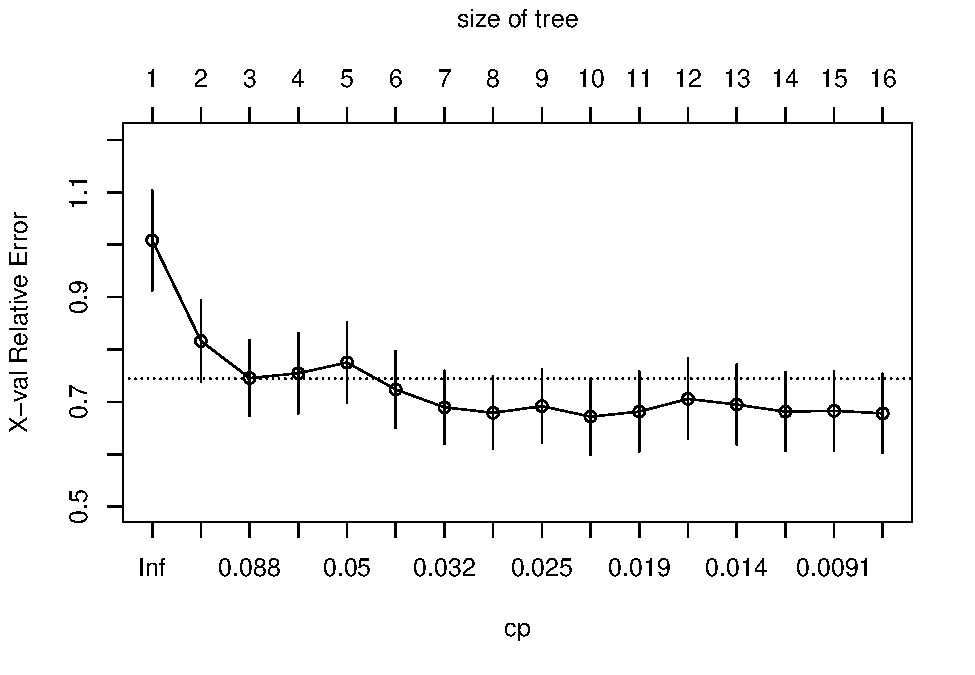
\includegraphics{A3_files/figure-latex/unnamed-chunk-5-1.pdf}

The test MSE is

\begin{verbatim}
## [1] 5.76
\end{verbatim}

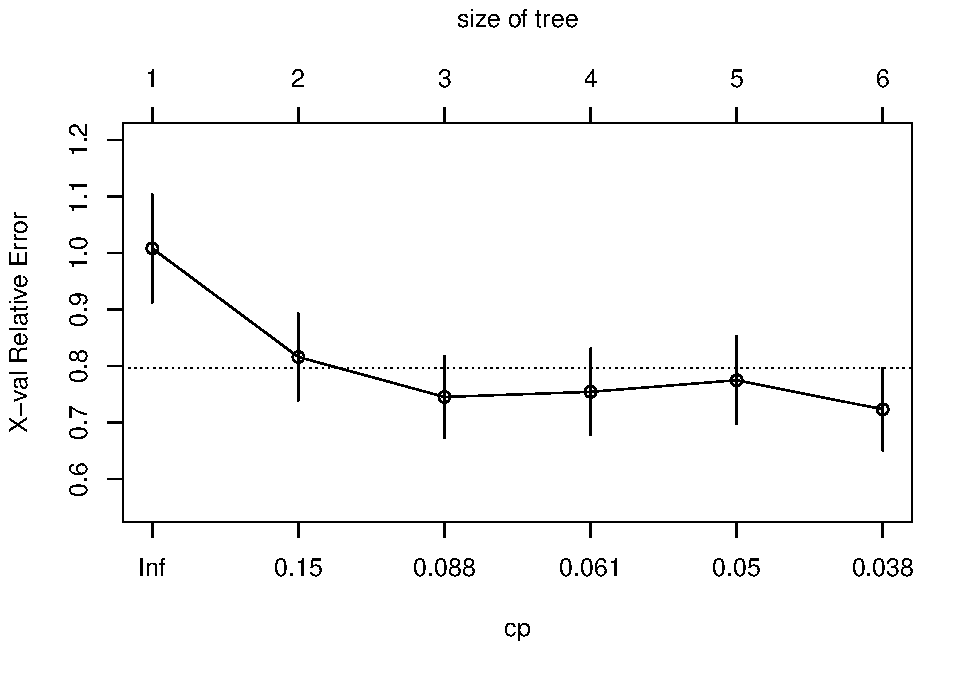
\includegraphics{A3_files/figure-latex/unnamed-chunk-7-1.pdf}

The test MSE with pruning is

\begin{verbatim}
## [1] 6.198
\end{verbatim}

\section{Exercise 2}\label{exercise-2}

We draw 100 observations from fourindependentvariables \(X_1\), \ldots{}
,\(X_4\) where

\begin{itemize}
  \item $X_1$ follows a uniform distribution,
  \item $X_2$ follows a standard normal distribution,
  \item $X_3$ follows a Bernoulli distribution with success probability $\pi$ = 0.5,
  \item $X_4$ follows a Bernoulli distribution with success probability $\pi$ = 0.1.
\end{itemize}

We repeat 1000 times the following:

\begin{itemize}
  \item Draw a dependent variable y from a standard normal distribution which is independent of the four independent variables.
  \item Fit a tree stump, i.e., a tree which contains only one split.
  \item Determine which variable was used for splitting.
\end{itemize}

Create the table of relative frequencies how often each of the variables
was selected for splitting. Given that all independent variables are not
associated with the dependent variable, is the probability of including
them as a split variable the same? If not, why would they differ?

\begin{verbatim}
## 
##    X1    X2    X3    X4 
## 0.460 0.471 0.037 0.032
\end{verbatim}

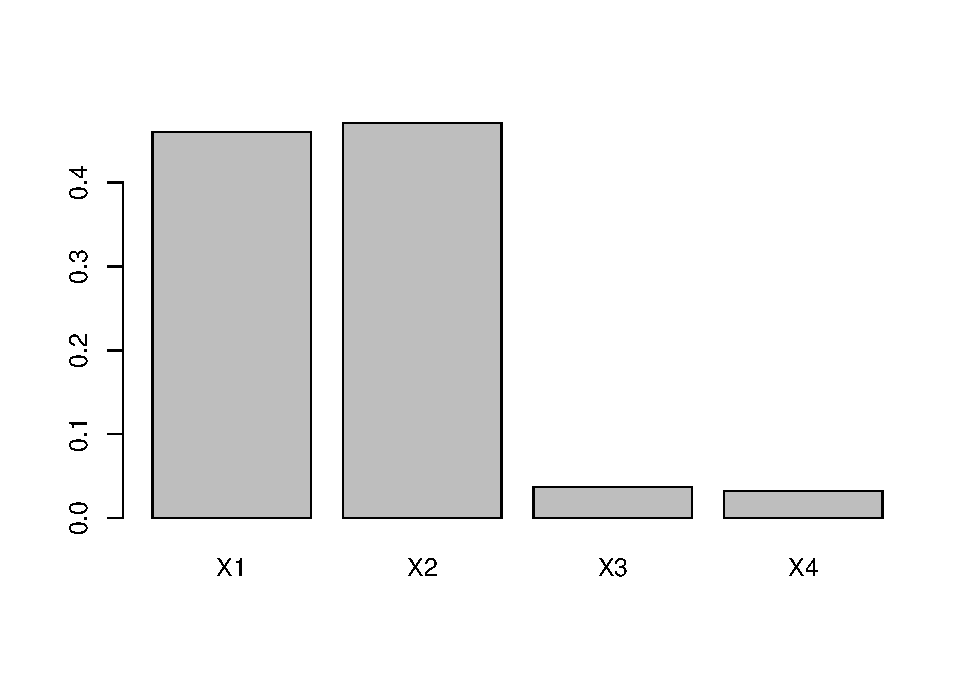
\includegraphics{A3_files/figure-latex/unnamed-chunk-10-1.pdf}

\section{Exercise 3}\label{exercise-3}

Let's assume the following data generating process
\[ Y = X + \epsilon, \] with \(X \sim N(0,1)\) and
\(\epsilon \sim N(0,1)\) independent. In addition 20 covariates
\(Z_1, ... ,Z_{20}\) are given with
\[Z_i \sim \sqrt{0.9}X + \epsilon Z_i ,\] where
\(\epsilon Z_i \sim N(0, 0.1).\)

We draw a training data with 30 observations and a test data with 10,000
observations from the data generating process including the additional
covariates \textbf{Z}.

We sample 100 bootstrap samples of size 30 from the training data of the
previous example by drawing with replacement.

Fit to each bootstrap sample:

\begin{enumerate}
\item a regression tree,
\item the null model with predicted value equal to the observed empirical mean of Y ,
\item a linear model including linear effects for X and all Z variables and
\item a linear model potentially including linear effects for X and all Z variables, but using model selection
with the AIC to select a suitable model starting from the null model.
\end{enumerate}

Determine the predicted values on the test data for the bagged model
estimator by calculating the average predictions over the 100 trees
fitted to the bootstrap samples, the 100 null models, the 100 linear
models including all linear effects and the 100 linear models based on
model selection.

\begin{verbatim}
##   Model   Mean
## 1  Tree 0.1912
## 2  Null 0.1847
## 3    LM 4.2230
## 4   AIC 0.3806
\end{verbatim}

Last, we determine the mean squared error of the four bagged model
estimators on the test sample of size 10,000.

\begin{verbatim}
##   Model    MSE
## 1  Tree  2.073
## 2  Null  2.070
## 3    LM 20.002
## 4   AIC  2.187
\end{verbatim}

\section{Exercise 4}\label{exercise-4}

We load the dataset icu in package \textbf{aplore3} which contains
information on patients who were admitted to an adult intensive care
unit (ICU). We develop a predictive model for the probability of
survival to hospital discharge of these patients. To fit a predictive
model to the data we use random forests.

We select a suitable number of bootstrap iterations.

Assess the influence of varying the hyperparameter m on the out-of-bag
error obtained and select a suitable value.

Inspect the variable importance measures. Compare the mean decrease Gini
and the mean decrease accuracy measures and assess if the observed
differences in relative importance assigned might be related to the
predictor variable being numeric or not.

\section{Exercise 5}\label{exercise-5}

Assume that there are four predictor variables which have the following
distributions:

\begin{align}
X_1 \sim N(0, 1),&& &X_2 \sim U(0, 1), \\
X_3 \sim M(1, (0.5, 0.5)),&& &X_4 \sim M(1, (0.2, 0.2, 0.2, 0.2, 0.2)).
\end{align}

This means we have two continuous variables which follow either a
standard normal or a standard uniform distribution (\(U(0, 1)\) and two
categorical variables with balanced categories with either 2 or 5
categories, i.e., \(M(N, \pi)\) is the multinomial distribution for N
trials and success probability vector \(\pi\). The dependent variable y
is assumed to be a binary categorical variable with equal-sized
classes.The sample size is set to N = 200.

We generate 100 datasets for each setting and fit a random forest to
each dataset and determine the mean decrease Gini and mean decrease
accuracy values for each of the predictor variables.

\begin{verbatim}
## randomForest 4.7-1.1
\end{verbatim}

\begin{verbatim}
## Type rfNews() to see new features/changes/bug fixes.
\end{verbatim}

Let's suitably visualize the results and interpret them.

\end{document}
